\protect\hyperlink{main-nav}{≡} \protect\hyperlink{close-nav}{×}

\hypertarget{section-2.9-applied-optimization}{%
\section{Section 2.9: Applied
Optimization}\label{section-2.9-applied-optimization}}

We have used derivatives to help find the maximums and minimums of some
functions given by equations, but it is very unlikely that someone will
simply hand you a function and ask you to find its extreme values. More
typically, someone will describe a problem and ask your help in
maximizing or minimizing something: ``What is the largest volume package
which the post office will take?''; ``What is the quickest way to get
from here to there?''; or ``What is the least expensive way to
accomplish some task?'' In this section, we'll discuss how to find these
extreme values using calculus.

\hypertarget{maxmin-applications}{%
\subsection{Max/Min Applications}\label{maxmin-applications}}

\hypertarget{example}{%
\paragraph{Example}\label{example}}

The manager of a garden store wants to build a 600 square foot
rectangular enclosure on the store's parking lot in order to display
some equipment. Three sides of the enclosure will be built of redwood
fencing, at a cost of \$7 per running foot. The fourth side will be
built of cement blocks, at a cost of \$14 per running foot. Find the
dimensions of the least costly such enclosure.

The process of finding maxima or minima is called optimization. The
function we're optimizing is called the \textbf{objective function} (or
\textbf{objective equation}). The objective function can be recognized
by its proximity to ``est'' words (greatest, least, highest, farthest,
most, \ldots{}). Look at the garden store example; the cost function is
the objective function.

In many cases, there are two (or more) variables in the problem. In the
garden store example again, the length and width of the enclosure are
both unknown. If there is an equation that relates the variables we can
solve for one of them in terms of the others, and write the objective
function as a function of just one variable. Equations that relate the
variables in this way are called \textbf{constraint equations}. The
constraint equations are always equations, so they will have equals
signs. For the garden store, the fixed area relates the length and width
of the enclosure. This will give us our constraint equation.

\hypertarget{max-min-story-problem-technique}{%
\paragraph{Max-Min Story Problem
Technique}\label{max-min-story-problem-technique}}

\begin{enumerate}
\item
  Translate the English statement of the problem line by line into a
  picture (if that applies) and into math. This is often the hardest
  step!
\item
  Identify the objective function. Look for words indicating a largest
  or smallest value.

  \begin{enumerate}
  \tightlist
  \item
    If you seem to have two or more variables, find the constraint
    equation. Think about the English meaning of the word
    ``constraint'', and remember that the constraint equation will have
    an equals sign.
  \item
    Solve the constraint equation for one variable and substitute into
    the objective function. Now you have an equation of one variable.
  \end{enumerate}
\item
  Use calculus to find the optimum values. (Take derivative, find
  critical points, test. Don't forget to check the endpoints!)
\item
  Look back at the question to make sure you answered what was asked.
  Translate your number answer back into English.
\end{enumerate}

Here is a link to the examples used in the videos in this section:
\href{otherfiles/applied_optimization_problems_math141.pdf}{Applied
Optimization Examples}.

To view this video please enable JavaScript, and consider upgrading to a
web browser that \href{http://videojs.com/html5-video-support/}{supports
HTML5 video}

\hypertarget{example-1}{%
\paragraph{Example 1}\label{example-1}}

The manager of a garden store wants to build a 600 square foot
rectangular enclosure on the store's parking lot in order to display
some equipment. Three sides of the enclosure will be built of redwood
fencing, at a cost of \$7 per running foot. The fourth side will be
built of cement blocks, at a cost of \$14 per running foot. Find the
dimensions of the least costly such enclosure.

First, translate line by line into math and a picture:

\begin{longtable}[]{@{}ll@{}}
\toprule
\endhead
\begin{minipage}[t]{0.47\columnwidth}\raggedright
\textbf{Text}\strut
\end{minipage} & \begin{minipage}[t]{0.47\columnwidth}\raggedright
\textbf{Translation}\strut
\end{minipage}\tabularnewline
\begin{minipage}[t]{0.47\columnwidth}\raggedright
The manager of a garden store wants to build a \emph{600 square foot
rectangular} enclosure on the store's parking lot in order to display
some equipment.

\emph{Three sides of the enclosure} will be built of redwood fencing, at
a \emph{cost of \$7 per running foot}. The \emph{fourth side} will be
built of cement blocks, at a \emph{cost of \$14 per running foot}.

Find the dimensions of the least costly such enclosure.\strut
\end{minipage} & \begin{minipage}[t]{0.47\columnwidth}\raggedright
Let \textbackslash{}(x\textbackslash{}) and
\textbackslash{}(y\textbackslash{}) be the dimensions of the enclosure,
with \textbackslash{}(y\textbackslash{}) being the length of the side
made of blocks. Then: \textbackslash{}{[}\textbackslash{}text\{Area\} =
A = xy = 600.\textbackslash{}{]}

\textbackslash{}(2x + y\textbackslash{}) costs \$7 per foot,
\textbackslash{}(y\textbackslash{}) costs \$14 per foot, so
\textbackslash{}{[}\textbackslash{}text\{Cost\} = C = 7(2x + y) + 14y =
14x + 21y.\textbackslash{}{]}

Find \textbackslash{}(x\textbackslash{}) and
\textbackslash{}(y\textbackslash{}) so that
\textbackslash{}(C\textbackslash{}) is minimized.\strut
\end{minipage}\tabularnewline
\bottomrule
\end{longtable}

\begin{figure}
\centering
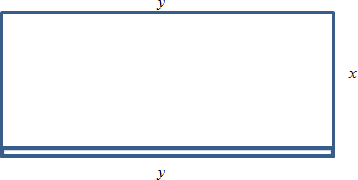
\includegraphics{images/image090.png}
\caption{}
\end{figure}

The objective function is the cost function, and we want to minimize it.
As it stands, though, it has two variables, so we need to use the
constraint equation. The constraint equation is the fixed area
\textbackslash{}(A = xy = 600\textbackslash{}). Solve
\textbackslash{}(A\textbackslash{}) for
\textbackslash{}(x\textbackslash{}) to get \textbackslash{}(
x=\textbackslash{}frac\{600\}\{y\} \textbackslash{}), and then
substitute into \textbackslash{}(C\textbackslash{}):
\textbackslash{}{[}C=14\textbackslash{}left(\textbackslash{}frac\{600\}\{y\}\textbackslash{}right)+21y=\textbackslash{}frac\{8400\}\{y\}+21y.\textbackslash{}{]}

Now we have a function of just one variable, so we can find the minimum
using calculus.

\textbackslash{}{[}C'=-\textbackslash{}frac\{8400\}\{y\^{}2\}+21\textbackslash{}{]}
\textbackslash{}(C'\textbackslash{}) is undefined for \textbackslash{}(y
= 0\textbackslash{}), and \textbackslash{}(C' = 0\textbackslash{}) when
\textbackslash{}(y = 20\textbackslash{}) or \textbackslash{}(y =
-20\textbackslash{}).

Of these three critical numbers, only \textbackslash{}(y =
20\textbackslash{}) makes sense (is in the domain of the actual
function) -- remember that \textbackslash{}(y\textbackslash{}) is a
length, so it can't be negative, and \textbackslash{}(y =
0\textbackslash{}) would mean there was no enclosure at all, so it
couldn't have an area of 600 square feet.

Test \textbackslash{}(y = 20\textbackslash{}) (here we chose the second
derivative test):
\textbackslash{}{[}C''=\textbackslash{}frac\{16800\}\{y\^{}3\}
\textbackslash{}gt 0,\textbackslash{}{]} so this is a local minimum.

Since this is the only critical point in the domain, this must be the
global minimum. Going back to our constraint function, we can find that
when \textbackslash{}(y = 20\textbackslash{}), \textbackslash{}(x =
30\textbackslash{}). The dimensions of the enclosure that minimize the
cost are 20 feet by 30 feet.

To view this video please enable JavaScript, and consider upgrading to a
web browser that \href{http://videojs.com/html5-video-support/}{supports
HTML5 video}

When trying to maximize their revenue, businesses also face the
constraint of consumer demand. While a business would love to see lots
of products at a very high price, typically demand decreases as the
price of goods increases. In simple cases, we can construct that demand
curve to allow us to maximize revenue.

\hypertarget{example-2}{%
\paragraph{Example 2}\label{example-2}}

A concert promoter has found that if she sells tickets for \$50 each,
she can sell 1200 tickets, but for each \$5 she raises the price, 50
less people attend. What price should she sell the tickets at to
maximize her revenue?

We are trying to maximize revenue, and we know that \textbackslash{}(
R=pq \textbackslash{}), where \textbackslash{}(p\textbackslash{}) is the
price per ticket, and \textbackslash{}(q\textbackslash{}) is the
quantity of tickets sold.

The problem provides information about the demand relationship between
price and quantity -- as price increases, demand decreases. We need to
find a formula for this relationship. To investigate, let's calculate
what will happen to attendance if we raise the price:

\begin{longtable}[]{@{}lllll@{}}
\toprule
\endhead
Price, \textbackslash{}( p \textbackslash{}) & 50 & 55 & 60 &
65\tabularnewline
Quantity, \textbackslash{}( q \textbackslash{}) & 1200 & 1150 & 1100 &
1050\tabularnewline
\bottomrule
\end{longtable}

You might recognize this as a linear relationship. We can find the slope
for the relationship by using two points:
\textbackslash{}{[}m=\textbackslash{}frac\{1150-1200\}\{55-50\}=\textbackslash{}frac\{-50\}\{5\}=-10.\textbackslash{}{]}

You may notice that the second step in that calculation corresponds
directly to the statement of the problem: the attendance drops 50 people
for every \$5 the price increases.

Using the point-slope form of the line, we can write the equation
relating price and quantity:
\textbackslash{}{[}q-1200=-10(p-50).\textbackslash{}{]}

Simplifying to slope-intercept form gives the demand equation
\textbackslash{}{[} q=1700-10p. \textbackslash{}{]}

Substituting this into our revenue equation, we get an equation for
revenue involving only one variable:
\textbackslash{}{[}R=pq=p(1700-10p)=1700p-10p\^{}2.\textbackslash{}{]}

Now, we can find the maximum of this function by finding critical
numbers. \textbackslash{}( R'=1700-20p \textbackslash{}), so
\textbackslash{}( R'=0 \textbackslash{}) when \textbackslash{}(p =
85\textbackslash{}).

Using the second derivative test, \textbackslash{}( R''=-20
\textbackslash{}lt 0 \textbackslash{}) (for any value of
\textbackslash{}( p \textbackslash{})), so the critical number is a
local maximum. Since it is the only critical number, we can also
conclude that it is the global maximum.

The promoter will be able to maximize revenue by charging \$85 per
ticket. At this price, she will sell \textbackslash{}( q=1700-10(85)=850
\textbackslash{}) tickets, generating \$72,250 in revenue.

To view this video please enable JavaScript, and consider upgrading to a
web browser that \href{http://videojs.com/html5-video-support/}{supports
HTML5 video}

To view this video please enable JavaScript, and consider upgrading to a
web browser that \href{http://videojs.com/html5-video-support/}{supports
HTML5 video}

\hypertarget{marginal-revenue-marginal-cost}{%
\subsection{``Marginal Revenue = Marginal
Cost''}\label{marginal-revenue-marginal-cost}}

You may have heard before that ``profit is maximized when marginal cost
and marginal revenue are equal.'' Now you can see why people say that!
(Even though it's not completely true.)

\hypertarget{example-3}{%
\paragraph{Example 3}\label{example-3}}

Suppose we want to maximize profit.

Now we know what to do -- find the profit function, find its critical
points, test them, etc.

But remember that Profit = Revenue - Cost. So Profit' = Revenue' -
Cost'. That is, the derivative of the profit function is
\textbackslash{}(MR - MC\textbackslash{}).

Now let's find the critical points -- those will be where Profit' = 0 or
is undefined. Profit' = 0 when \textbackslash{}(MR - MC =
0\textbackslash{}), or where \textbackslash{}(MR = MC\textbackslash{}).

Profit has critical points when Marginal Revenue and Marginal Cost are
equal.

In all the cases we'll see in this class, Profit will be very well
behaved, and we won't have to worry about looking for critical points
where Profit' is undefined. But remember that not all critical points
are local max! The places where \textbackslash{}(MR =
MC\textbackslash{}) could represent local max, local min, or neither
one.

\hypertarget{example-4}{%
\paragraph{Example 4}\label{example-4}}

A company sells \textbackslash{}(q\textbackslash{}) ribbon winders per
year at \textbackslash{}(\textbackslash{}\$p\textbackslash{}) per ribbon
winder. The demand function for ribbon winders is given by:
\textbackslash{}(p=300-0.02q\textbackslash{}). The ribbon winders cost
\$30 apiece to manufacture, plus there are fixed costs of \$9000 per
year. Find the quantity where profit is maximized.

We want to maximize profit, but there isn't a formula for profit given.
So let's make one. We can find a function for Revenue =
\textbackslash{}(pq\textbackslash{}) using the demand function for
\textbackslash{}(p\textbackslash{}).
\textbackslash{}{[}R(q)=(300-0.02q)q=300q-0.02q\^{}2.\textbackslash{}{]}

We can also find a function for Cost, using the variable cost of \$30
per ribbon winder, plus the fixed cost:
\textbackslash{}{[}C(q)=9000+30q.\textbackslash{}{]}

Putting them together, we get a function for Profit:
\textbackslash{}{[}P(q)=R(q)-C(q)=\textbackslash{}left(300q-0.02q\^{}2\textbackslash{}right)-(9000+30q)=-0.02q\^{}2+270q-9000\textbackslash{}{]}

Now we have two choices. We can find the critical points of Profit by
taking the derivative of \textbackslash{}(P(q)\textbackslash{})
directly, or we can find \textbackslash{}(MR\textbackslash{}) and
\textbackslash{}(MC\textbackslash{}) and set them equal. (Naturally,
we'll get the same answer either way.)

Let's use \textbackslash{}(MR = MC\textbackslash{}) this time.
\textbackslash{}{[} \textbackslash{}begin\{align*\} MR=\&
300-0.04q\textbackslash{}\textbackslash{} MC=\&
30\textbackslash{}\textbackslash{} 300-0.04q=\&
30\textbackslash{}\textbackslash{} 270=\&
0.04q\textbackslash{}\textbackslash{} q=\& 6750
\textbackslash{}end\{align*\} \textbackslash{}{]}

The only critical point is at \textbackslash{}(q =
6750\textbackslash{}). Now we need to be sure this is a local max and
not a local min. In this case, we'll look to the graph of
\textbackslash{}(P(q)\textbackslash{}) -- it's a downward opening
parabola, so this must be a local max. And since it's the only critical
point, it must also be the global max.

Profit is maximized when they sell 6750 ribbon winders.

To view this video please enable JavaScript, and consider upgrading to a
web browser that \href{http://videojs.com/html5-video-support/}{supports
HTML5 video}

\hypertarget{average-cost-marginal-cost}{%
\subsection{``Average Cost = Marginal
Cost''}\label{average-cost-marginal-cost}}

``Average cost is minimized when average cost = marginal cost'' is
another saying that isn't quite true; in this case, the correct
statement is:

Average Cost has critical points when Average Cost and Marginal Cost are
equal.

Let's look at a geometric argument here. Remember that the average cost
is the slope of the diagonal line, the line from the origin to the point
on the total cost curve. If you move your clear plastic ruler around,
you'll see (and feel) that the slope of the diagonal line is smallest
when the diagonal line just touches the cost curve -- when the diagonal
line is actually a tangent line -- when the average cost is equal to the
marginal cost.

\begin{figure}
\centering
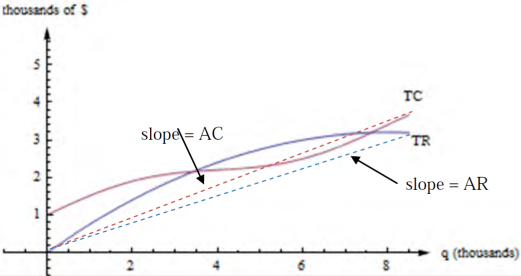
\includegraphics{images/image113.png}
\caption{}
\end{figure}

To view this video please enable JavaScript, and consider upgrading to a
web browser that \href{http://videojs.com/html5-video-support/}{supports
HTML5 video}

\begin{longtable}[]{@{}ll@{}}
\toprule
\endhead
\href{section2-8.php}{← Previous Section} & \href{section2-10.php}{Next
Section →}\tabularnewline
\bottomrule
\end{longtable}
